% !TEX root = ../../main.tex


\begin{figure}[p]
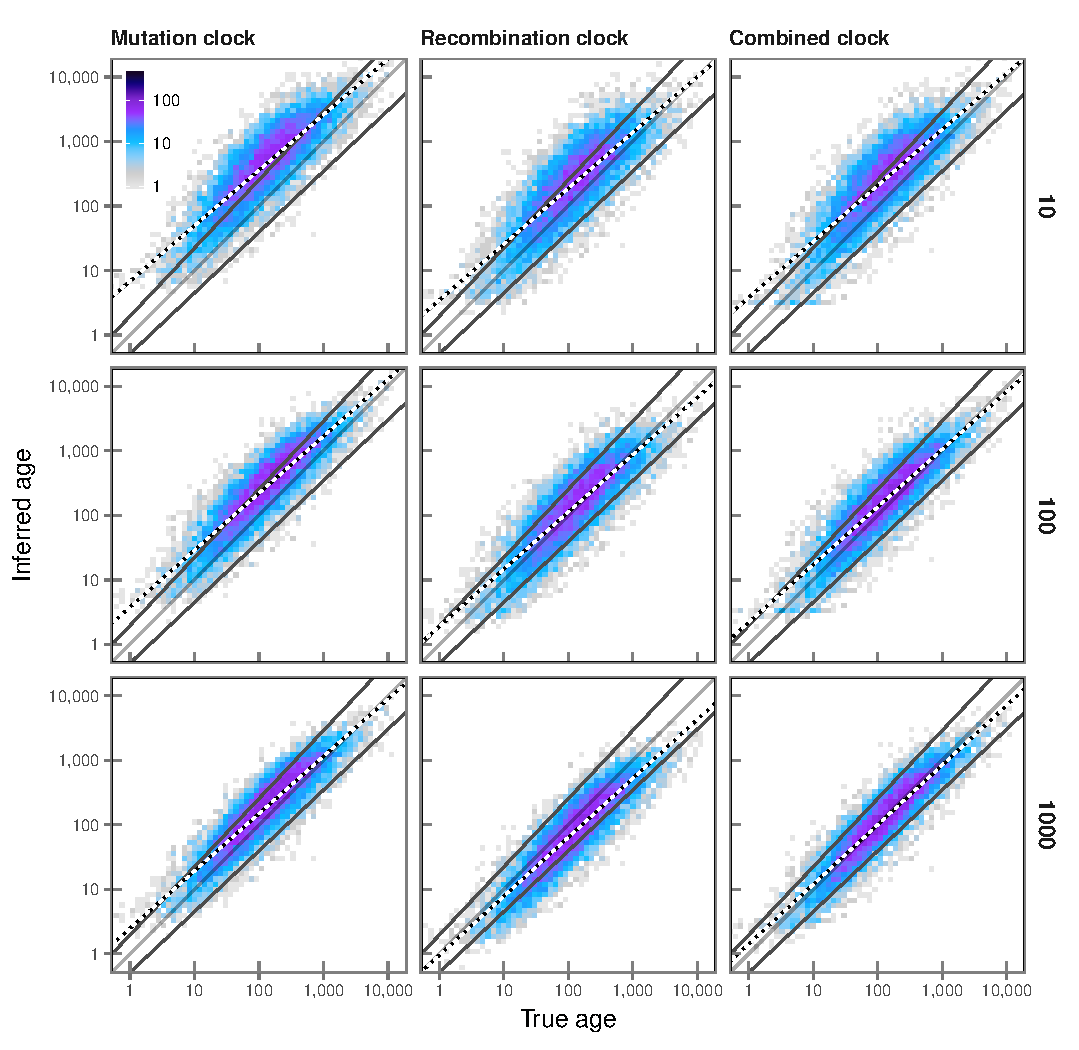
\includegraphics[width=\textwidth]{./img/ch5/discords_scat}
\Caption{True and inferred age under varying numbers of discordant pairs}
{A set of \n{10000} target sites was randomly drawn in \fk{[2,20]} (shared allele frequency ${\leq 1\%}$) in a simulated sample of \n{2000}~haplotypes.
Different numbers of sampled discordant pairs were analysed on the same set of target variants, which is shown for ${n_d = \num{10}}$, ${n_d = \num{100}}$, and ${n_d = \num{1000}}$ (indicated at the \emph{right} of each row).
True IBD was used to estimate allele age.
IBD breakpoints were determined from simulation records and defined as the first variant sites observed in the data following the \n{2} recombination events on each side of a given focal position.
Age was estimated under each of the \n{3} clock models; \ie mutation clock, \ClockM, recombination clock, \ClockR, and combined clock, \ClockC (indicated at the \emph{top} of each column).
Each panel shows the density distribution of true and inferred age (numbers indicated by the colour-gradient).
The true age of a focal allele was set at $t_m$, which is the geometric mean of $t_c$ and $t_d$, \ie the true time of the coalescent event from which the focal allele derived ($t_c$) and the true time of the coalescent event immediately preceding that event ($t_d$) in the history of the sample; these are indicated by their linear regression trend lines \emph{below} and \emph{above} the dividing line at $t_m$, respectively.
The \emph{black-white} line indicates the line of best fit resulting from linear regression of age estimates, using the posterior mode of the composite likelihood distribution as the inferred age value.
Note that both true and inferred age are compared on log-scale, as the time to a coalescent event is expected to increase exponentially back in time.}
{fig:discords_scat}
\end{figure}
